\documentclass[12pt, a4paper, openany]{book}
\usepackage[italian]{babel}
\usepackage{listings}
\usepackage{graphicx}
\usepackage{fancyvrb}
\usepackage{amssymb}
\usepackage{amsmath}
\usepackage{hyperref}
\graphicspath{ {./images/} }

\begin{document}
\title{PES - Probabilità e Statistica per l'informatica}
\author{Elia Ronchetti}
\date{Marzo 2022}

\maketitle
\tableofcontents

\chapter{Introduzione}
Il corso di probabilità e statistica per l'informatica è diviso in 2 parti
\begin{enumerate}
    \item Stastica Descrittiva - Descrivere e riassumere i dati
    \begin{enumerate}
        \item Probabilità - Descrivere matematicamente i fenomeni casuali
    \end{enumerate}
    \item Statistica inferenziale - Trarre conclusioni dai dati
\end{enumerate}

%Modalità d'esame
\chapter{Esame}
L'esame sarà strutturato nella seguente maniera
\paragraph{Parte 1 - Teoria}
8 Domande a risposta multipla - Punteggio 10/30
\paragraph{Parte 2 - Pratica}
4 Esercizi a risposta aperta - Punteggio 20/30
\paragraph{Progetto (facoltativo)}
Progetto R, da consegnare prima dell'esame, può fornire un massimo di 2/30

\chapter{Analisi Descrittiva}
\section{Descrivere i dati}
Per descrivere una raccolta dati in maniera chiara e immediata è utile utilizzare una \textbf{tabella delle frequenze}
all'interno della quale sono contenuti:
\begin{itemize}
    \item Valori
    \item Frequenze Assolute - Numero di volte in cui compare "i" nell'insieme di dati
    \item Frequenze Relative - Frazione di volte in cui compare i nell'insieme di dati
    \item Percentuali - (Frequenza relativa x 100)
\end{itemize}

Il dato che compare con frequenza più alta è detto \textbf{moda}.

I dati possono essere
\begin{itemize}
    \item Qualitativi
    \item Quantitativi 
\end{itemize}
Noi useremo i dati \textbf{quantitativi}

\subsection{Rappresentazione dei dati}
Per rappresentare le frequenze (assolute o relative) risulta efficace e immediato l'utilizzo di un grafico a barre detto istogramma,
esso rappresenta in graficamente la tabella, chiaramamente da esso è possibile risalire alla tabella stessa.
Capita di avere degli insiemi di dati che assumono un valore elevato di valori distini, per questo conviene suddividerli in classi e
determinare la frequenza di ciascuna classe. In questo modo c'è una perdita d'informazioni (sui valori specifici), ma così facendo possiamo
calcolare le frequenze delle classi e avere un'idea migliore della distribuzione dei dati.

\subsection{Dati Bivariati}
Quando per ciascun individuo vengono misurate due variabili ci troviamo un insieme di N dati a coppie detti \textbf{dati bivariati}.
Anche in questo caso è possibile calcolare le frequenze, in questo caso detto \textbf{frequenze congiunte}.

è possibile, inoltre, misurare la correlazione tra le due variabili attraverso per esempio un diagramma di dispersione (detto anche scatterplot).

\paragraph{Correlazione non significa causalità!} Non è detto che l'aumento di una variabile causi la diminuzione dell'altra o viceversa, potrebbe esserci una causa comune. 

\section{Riassumere i dati}
Dopo aver rappresentato i dati vogliamo ora riassumerli mediante quantità numeriche, dette \textbf{Statistiche Campionarie}, al fine di sintetizzare le proprietà
salienti dei dati.

\subsection{Indici di posizione}
Per definire il centro dell'insieme dei dati definiamo la 
\paragraph{\textbf{Media Campionaria}} \scalebox{1.5}{$\frac{x_1 + x_2 + \dots + x_n}{N}$} %Aggiungere sommatoria

Per misurare il valore in posizione centrale (considerando l'insieme di dati ordinato), utilizziamo la
\paragraph{\textbf{Mediana}}
\begin{itemize}
    \item Se N dispari $\rightarrow$ {$X_\frac{N+1}{2}$}
    \item Se N pari $\rightarrow$ $m = \frac{X_{\frac{N}{2}}+X_{\frac{N}{2}+1}}{2}$
\end{itemize}

La mediana è insesibile alle code, se per esempio quindi aumento anche di molto il valore dell'ultima cifra lasciando invariate
le altre la mediana non cambierà (a differenza della media).

\section{Coefficiente di correlazione lineare}
Posso misurare il grado di correlazione tra una coppia di dati attraverso il coefficiente di correlazione lineare. 

\begin{equation}
    r = \frac{\sum_{k=1}^N (x_i - x)(y_i - y)}{(N -1)S_x S_y}
\end{equation}

Si può mostrare che:
\begin{equation}
    -1<=r<=1
\end{equation}

In generale $r > 0$ indica una correlazione positiva
\\ $r < 0$ indica una correlazione negativa 

\subsection{Correlazioni significative}
$|r| > 0.7$ Correlazione significativa
\\$|r| < 0.3$ Correlazione debole

\section{Percentili e quantili}
Per analizzare la distribuzione dei dati è utile fissare un numero k che rappresenta la posizione all'interno dato all'interno dell'insieme
questo valore percentuale è detto \textbf{k-esimo Percentile Campionario}, valore t per cui
\begin{itemize}
    \item almeno il k\% dei dati è $ <= t$
    \item almeno il $(100 -k)\%$ dei dati è $<= t$
\end{itemize}

I casi più importanti sono per k = 25, 50, 75
\\ Risulta pratico scrivere $k = 100p$ dove $p = \frac{k}{100}\in [0, 1]$, dove i casi importanti sono per:
\begin{itemize} 
    \item $p = \frac{1}{4}: k = 100p$ = 25-esimo percentile = primo quartile $q_1$
    \item $p = \frac{1}{2}: k = 100p$ = 50-esimo percentile = secondo quartile $q_2$ = mediana m
    \item $p = \frac{3}{4}: k = 100p$ = 75-esimo percentile = terzo quartile $q_3$
\end{itemize}

Per calcolare il k-esimo percentile t è necessario:
\begin{enumerate}
    \item Ordinare l'insieme di dati $x_1 <= x_2 <= \dots <= x_n$
    \item Se $N_p$ non è intera $t=x_i$ è il dato la cui posizione i è l'intero successivo a $N_p$
    \item Se $N_p$ è intera $t = \frac{x_(Np) x_(Np+1)}{2}$ è la media aritmetica fra il dato in posizione N e il successivo 
\end{enumerate}

\paragraph{Nota per R} Esistono diverse definizioni di quantile, R per esempio ne utilizza una diversa di default.

\'E possibile utilizzare i \textbf{Boxplot} per la rappresentazione dei quantili

\chapter{Probabilità}
Il calcolo delle probabilità è la teoria matematica che permette di descrivere e studiare \textbf{esperimenti aleatori}
\paragraph{Esperimento aleatorio} $\to$ Fenomeno il cui esito non è prevedibile con certezza a priori
\section{Introduzione}
La descrizione matematica si articola in tre passi
\begin{enumerate}
    \item Spazio campionario (o spazio degli esiti)$\to$ Insieme $\Omega$ che contiene tutti i possibili esiti dell'esperimento \\ es. Tiro un dado a sei facce $\Omega = {1, 2, 3, 4, 5, 6}$
    \item Eventi $\to$ sono i sottinsiemi dello spazio campionario $A \subseteq \Omega$ \\ es. Tiro un dado a sei facce: esce un numero pari $A = {2, 4, 6}$
    \item Probabilità $\to$ Regola che assegna, in modo coerente, a ogni evento $A \subseteq \Omega$ un "grado di fiducia" $P(A)$, tra 0 e 1, che attribuiamo al verificarsi di A
    O funzione $P: P(\Omega) \to [0, 1]$ che soddisfa opportune proprietà
\end{enumerate}
\section{Proprietà di base} 
\begin{enumerate}
    \item $P(\Omega) = 1$
    \item Se A e B sono eventi disgiunti, cioè $A \cap B \neq \emptyset$, allora \\ $P (A \cup B) = P(A) + P(B)$
\end{enumerate}
\paragraph{La coppia $(\Omega, P)$ è detta \textbf{Spazio di Probabilità}}.
\\ Fissiamo uno spazio di probabilità $(\Omega, P)$.
Da queste proprietà si deducono molte altre proprietà
\begin{itemize}
    \item $P(\emptyset) = 0$
    \item \textbf{Regola del complementare} $\to P(A^c) = 1 - P(A)$ \\ Vale per ogni A
    \item \textbf{Regola della addizione di probabilità} $\to P(A \cup B) = P(A) + P(B) - P(A \cap B)$ 
    \\ Vale per ogni A, B (anche $A \cap B \neq \emptyset$)
    \item Monotonia: se $A \subseteq B$ allora $P(A) <= P(B)$
\end{itemize}
\paragraph{Analogia} c'è un analogia tra probabilità e area
\begin{center}
    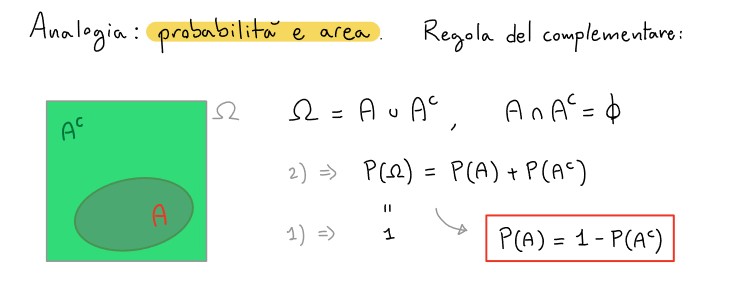
\includegraphics[width=120mm,scale=0.5]{analogia_prob_area.png}
\end{center}

\section{Calcolo combinatorio}
Consideriamo uno spazio di probabilità uniforme $(\Omega, P)$
\begin{itemize}
    \item $P(A) = \frac{|A|}{|\Omega|}$ = $\frac{Casi favorevoli}{Casi Possibili}$
    per ogni $A \subseteq \Omega$
    \item $P({w}) = \frac{1}{\Omega} = \frac{1}{n}$ per ogni $w \in \Omega$
\end{itemize}
Questo è il modello appropriato per descrivere esperimenti aleatori i cui esiti
siano tutti equiprobabili. Quando scegliamo casualmente una persona/oggetto in un 
insieme finito senza ulteriori specifiche, si sottintende che la scelta è effettuata
in modo uniforme.
Affinchè la probabilità uniforme sia ben definita, lo spazio campionario $\Omega$
deve essere finito (se così non fosse la probabilità uniforme su $\Omega$ non esiste)
\\ In uno spazio di probabilità uniforme calcolare una probabilità significa contare gli 
elementi di un insieme
\begin{equation}
    P(A) = \frac{|A|}{|\Omega|}
\end{equation}
Dato che contare non è banale per insiemi grandi sono nate tecniche di conteggio,
esse formano il \textbf{Calcolo Combinatorio}
\paragraph{Principio Fondamentale} Consideriamo un esperimento costituito da due parti:
\begin{enumerate}
    \item n esiti possibili
    \item m esiti possibili
\end{enumerate}
L'esperimento totale può avere $n*m$ esiti possibili.
\paragraph{Esempio} Il lancio dei dadi. Se lancio 2 dadi a sei facce ho $\Omega$ 
esiti possibili
\begin{equation}
    |\Omega| = 6*6 = 36
\end{equation}
\subsection{Disposizioni con ripetizione}
Sequenze ordinate di k elementi (anche ripetuti) scelti tra n possibili. Numero totale è:
\begin{equation}
    n*n \dots n = n^k
\end{equation}
\paragraph{Esempio} Estrazione casuale di 3 persone, calcolare la probabilità che
siano tutte nate in primavera.
In questo caso lo spazio campionario sono i compleanni delle tre persone quindi
\begin{equation}
    \Omega = {(x_1, x_2, x_3): x_1, x_2, x_3 \text{ in Calendario}}
\end{equation}
Questa è una disposizione con ripetizione di 3 elementi estratti dal calendario
\begin{equation}
    |\Omega| = 365*365*365 = 365^3
\end{equation}
Probabilità uniforme $P(A) = \frac{|A|}{|\Omega|}$
\\ In questo caso tutti i nati in primavera vengono considerati 
nati A = tutti  nati in primavera = [20 marzo, 21 giugno) e in totale sono 92 giorni.
\\ Si tratta anche qua di una disposizione ripetuta di 3 elementi.
\begin{equation}
    |A| = 92*92*92 = 92^3
\end{equation}
Per calcolare la probabilità è sufficiente dividere A per $\Omega$
\begin{equation}
    P(A) = \frac{|A|}{|\Omega|} = \frac{92^3}{365^3} = 0,016 = 1,6\%
\end{equation}
Se avessi estratto k persone sarebbe stato sufficiente sostituire l'esponente con k.

\subsection{Disposizioni semplici}
Sequenze ordinate di k elementi distinti scelti tra n possibili (con $k <= n$) 
\textbf{senza ripetizione}
\begin{equation}
    n*(n-1)*(n-2)\dots(n-k+1) = \frac{n!}{(n-k)!}
\end{equation}
\'E preferibile utilizzare la prima formula su R dato che il fattoriale scala molto male,
su carta spesso si semplifica, ma su Computer si calcolerebbe tutto il fattoriale e spesso richiede 
molto tempo.
\\ Se $k = n$ si parla di \textbf{Permutazioni} di n oggetti. In numero sono:
\begin{equation}
    n! = n*(n-1)*(n-2)\dots 2 * 1
\end{equation}
\paragraph{Esempio}. Quanti sono i possibili ordini di arrivo di 3 squadre?
Si tratta di una permutazione di 3 elementi.
\paragraph{Esempio Paradosso dei compleanni}

\subsection{Combinazioni}
In molti casi non siamo interessati all'ordine. 
Per esempio, se dobbiamo scegliere un comitato di 2 persone non ci interessa l'ordine 
dei candidati.
Si parla in questo caso di combinazioni, esse si possono ottenere dalle disposizioni semplici
"dimenticando" l'ordine degli elementi.
\begin{equation}
    {n \choose x} = \frac{n!}{k!(n-k)!}
\end{equation}
Insiemi = collezioni (non ordinate) di k elementi distinti scelti tra n possibili (con $k <= n$).
\paragraph{Esempio}. Mano di carte a Poker, un giocatore riceve 5 carte estratte da un mazzo che
ne contiene 52. Il numero di possibili mani è
\begin{equation}
    {52 \choose 5} = \frac{52!}{5!47!}
\end{equation} 

\section{Probabilità Condizionata}
Consideriamo un esperimento aleatorio, che descriviamo con uno spazio di probabilità $(\Omega, P)$.
Consideriamo un evento $A \subseteq \Omega$, che ha un probabilità $P(A)$.
Supponiamo di ricevere l'informazione che un altro evento B si è verificato.
Come è ragionevole aggiornare la probabilità di A per tenere conto di questa informazione aggiuntiva?
\\La soluzione è data dalla probabilità Condizionata.
\begin{equation}
    P(A|B) = \frac{P(A \cap B)}{P(B)}
\end{equation}
La precedente formula denota la probabilità condizionata di A dato B (o sapendo B).
Sto quindi calcolando la probabilità di A.
\begin{center}
    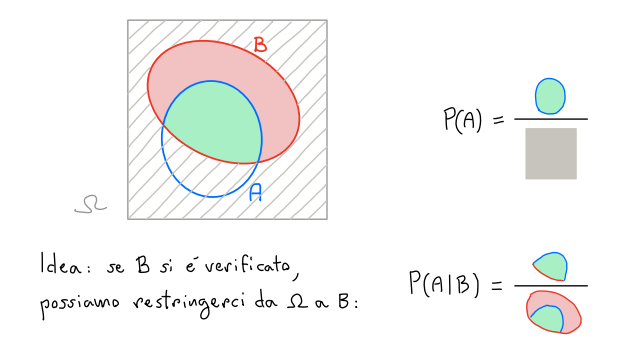
\includegraphics[width=120mm,scale=0.5]{prob_condizionata_area.png}    
\end{center}
Quando si verifica un evento lo spazio di probabilità si riduce (vedere esempio sui dadi)
\subsection{Regola del prodotto}
\begin{equation}
    P(A \cap B) = P(A)*P(B|A)
\end{equation}
\subsection{Formula di Disintegrazione}
\begin{equation}
    P(A) = P(A \cap B) + P(A \cap B^c)
\end{equation}
\subsection{Formula delle probabilità totali}
\begin{equation}
    P(A) = P(A|B)*P(B) + P(A|B^c)*P(B^c)
\end{equation}
Inoltre $P(*|B)$ + una probabilità, in particolare:
\begin{equation}
    P(A^c|B) = 1 - P(A|B)
\end{equation}
\subsection{Formula di Bayes}
\begin{equation}
    P(B|A) = \frac{P(A|B)*P(B)}{P(A)}
\end{equation}
\paragraph{Esempio}. Per vedere la parte pratica andare a vedere l'esempio sui tamponi
per rilveare la presenza di un virus. Super interessante e utile.
\\Il file è \textbf{Appunti Lezione 3 - In fondo al PDF}

\section{Indipendenza di eventi}
Può capitare che, per un evento A, l'informazione che un altro evento B si è verificato
non ne cambi la probabilità.
\begin{equation}
    P(A|B) = P(A)
\end{equation}
che equivale
\begin{equation}
    P(A \cap B) = P(A)*P(B)
\end{equation}
In questo caso gli eventi A e B si dicono \textbf{Indipendenti}
\paragraph{Esempi}
Lancio di due dadi, i risultati sono eventi indipendenti
\\ Urna contenente 5 palline rosse e 3 palline verdi. Pesco in successione due palline, 
senza reimmissione. La probabilità che la prima pallina sia rossa e che la seconda sia rossa
sono \textbf{dipendenti}!

\subsection{Eventi indipendenti != Eventi disgiunti!}
\begin{center}
    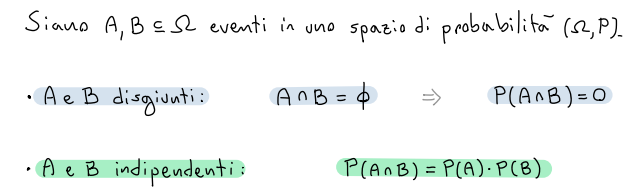
\includegraphics[width=120mm, scale=0.5]{differenza_disgiunti_indipendenti.png}
\end{center}
Quindi due eventi indipendenti non possono essere disgiunti,
tranne nel caso "banale" in cui uno dei due abbia probabilità
nulla.

\paragraph*{Esempio} Una famiglia ha due figli/e descritti da 
\\ $\Omega = \{MM, FF, FM, FF\}$ e $P=\text{Probabilità uniforme} = \frac{1}{4}$
\\ Consideriamo gli eventi:
\begin{itemize}
    \item A := "il primo genito è maschio" = \{MM, FF\}
    \item B := "il secondo genito è maschio" = \{MM, FM\}
    \item C := "la primogenita è femmina" =\{FM, FF\}
\end{itemize}
\begin{center}
    In questo caso A e B sono \textbf{indipendenti}, ma \textbf{NON disgiunti};
\\ A e C sono \textbf{disgiunti}, ma \textbf{NON indipendenti}.
\end{center}

\paragraph{Estensioni}
Tre eventi A, B, C si dicono indipendenti se valgono
\begin{center}
    $P(A \cap B \cap C) = P(A)P(B)P(C)$
    \\$P(A \cap B) = P(A)P(B)$
    \\$P(B \cap C) = P(B)P(C)$
    \\$P(A \cap C) = P(A)P(C)$
\end{center}

% Variabili Aleatorie
\chapter{Variabili aleatorie}
Variabile aleatoria (detta anche casuale o stocastica), è una variabile che può assumere valori
diversi in dipendenza da qualche fenomeno aleatorio. Il termine "aleatorio" deriva dal latino \textit{alea} (gioco di dadi), ed esprime il
concetto di rischio calcolato.
\begin{center}
    \textit{"alea iacta est"} - "il dado è tratto"
\end{center}

Consideriamo un esperimento aleatorio, descritto da uno spazio di probabilità $(\Omega, P)$.
Spesso non siamo interessati a tutti i dettagli del'esito dell'esperimento, ma solo a 
una quantità (tipicamente numerica) determinata dall'esito dell'esperimento.
Una tale quantità è detta \textbf{Variabile aleatoria}.
\\ Possiamo considerare la variabile aleatoria come:
\begin{itemize}
    \item Intero: Quantità che dipende dal "caso"
    \item Funzione matematica: Funzione definita sullo spazio campionario: $X: \Omega \to R$
\end{itemize}
Ricodiamo che un evento è:
\begin{itemize}
    \item Affermazione sull'esito dell'esperimento aleatorio
    \item Sottoinsieme dello spazio campionario: $A \subset \Omega$
\end{itemize}

Se X è una variabile aleatoria, e se x è un suo possibile valore, allora:
\begin{itemize}
    \item o X assume il valore x
    \item oppure ${w \in \Omega: X(w) = x }$
\end{itemize}

Ogni variabile aleatoria X determina molti eventi!
\paragraph{Attenzione}: non confondere variabili aleatorie ed eventi
\\ Le variabili aleatorie rappresentano esiti esprimibili numericamente di esperimenti
ancora da effettuare! Dove per esperimento si intende qualsiasi fenomeno o situazione con sviluppi
imprevedibili a priori. Essendo imprevedibile a priori il valore assunto da una variabile
aleatoria, tutto ciò che si può fare è esprimere delle valutazioni di tipo probabilistico sui valori
che essa assumerà. Per questa ragione ad ogni variabile aleatoria X è associata una funzione che esprime
in modo chiaro tali valutazioni. 
\\Se la variabile è discreta si parlerà di \textbf{Densità discreta}.
\\Se la variabile è continua di parlerà di \textbf{Funzione di ripartizione}.

\section{Notazione} Con $X_i$ indichiamo la Variabile Aleatoria $X_i: \Omega \rightarrow \mathbb{R}$
\\ con $x_i$ indichiamo l'osservazione relativa alla V.A $X$

\section{Variabili aleatorie discrete}
Una variabile aleatoria X (reale) si dice \textbf{discreta} se i valori che può
assumere sono un insieme finito:
\begin{equation}
    X(\Omega) = {x_1, x_2, \dots, x_n} \subseteq  R
\end{equation}
Oppure un insieme infinito numerabile
\begin{equation}
    X(\Omega) = {x_1, X_2, \dots } = {x_i} i \in N \subseteq R
\end{equation}
Ad ogni variabile aleatoria discreta X possiamo associare
\begin{center}
    \textbf{Densità discreta} $P_x(x_i) = P(X = x_i)$
\end{center}
Definita anche come distribuzione di probabilità, è una funzione che assegna
ad ogni valore possibile di X la probabilità dell'evento elementare $(X = x)$
\subsection{Proprietà}
\begin{center}
    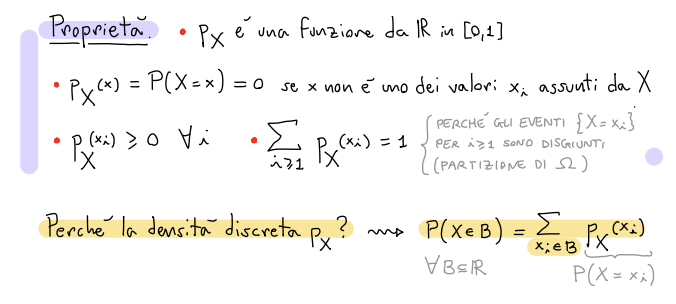
\includegraphics[width=120mm, scale=0.5]{prop_densità_discreta.png}
\end{center}
Concettualmente una v.a. (variabile aleatoria) X è rappresentata matematicamente da una
una funzione definita sullo spazio campionario $\Omega$ di un esperimento aleatorio.
\begin{center}
    $X:\Omega \to R$
\end{center}
Allo stesso tempo possiamo pensare a X come a un numero che dipende dal caso.
Se siamo interessati a una v.a. discreta X, spesso non è necessario scrivere lo
spazio campionario $\Omega$ ed esprimere X come funzione, 
ci basta conoscere la densità discreta.

\subsection{Valore medio di X}
Sia X una variabile aleatoria discreta (reale) che assume una quantità finita di valori
$x_1, x_2, \dots, x_n$. Si definisce

\begin{equation}
    E[X]:= \sum_{i = 1}^{n} x_i (p_X)^{x_i} = \sum_{i = 1}^{n} x_i P(X= x_i)
\end{equation}
\paragraph{Valore Medio} è la somma dei valori assunti da X "pesati" con le rispettive probabilità.

\paragraph*{Esempio figli}In poche parole se ripetiamo tante volte l'esperimento e ne calcoliamo la media otteniamo
il valore medio, per esempio il valore medio della v.a. "X = numero di figli maschi"
su una coppia con 2 figli è 1, perchè mediamente una coppia con 2 figli ha almeno 1 figlio maschio.

\paragraph*{Esempio dado} Sia "X = risultato del lancio di un dado regolare a 6 facce".
$E[X] = 3.5$. 
\\ Non è un valore assunto dalla v.a. dato che i numeri sul dado sono solo interi.
\\ Si può notare dall'esempio precedente che il valore medio E[X] non è necessariamente
uno dei valori $x_i$ assunti da X!
A maggior ragione, E[X] non è un valore tipico di X, nè un valore che necessariamente
ci aspettiamo di osservare.
\\ Ma allora qual è l'interpretazione del valore medio $E[X]$? A cosa serve?
\\ Di seguito è riportata l'interpretazione frequentista di E che spiega a livello
pratica cosa rappresenta.

\subsubsection{Interpretazione frequentista di E[X]}
Supponendo di ripetere l'esperimento aleatorio un numero elevato di volte $N >> 1$
e indicando con $X_1, X_2, \dots, X_n$ le variabili aleatorie che rappresentano X nelle
ripetizioni dell'esperimento si ha con grande probabilità che:
\begin{equation}
    \frac{X_1 + X_2 + \dots + X_n}{N} \backsimeq  E[X]
\end{equation}

\subsection{Proprietà del valore medio}
Per ogni variabile aleatoria (reale) X
\begin{center}
    $E[X + c] = E[X] + c$
    \\$E[cX] = c E[X]$
\end{center}
Questo vale per ogni costante $c \in R$
\\ Se X e Y sono due variabili aleatorie che dipendono entrambe dallo
stesso esperimento aleatorio, allora:
\begin{center}
    $E[X+Y] = E[X] + E[Y]$
\end{center}
Si dice che il valore medio è un operatore lineare.
\paragraph{Altre importanti proprietà} Se $X = c$ (costante) allora
$E[X] = E[c] = c$
\\ Un'altra proprietà importante: Se $X >= 0$ allora $E[X] >= 0$
\paragraph{Formula di trasferimento} 

\begin{equation}
    E[f(x)] = \sum_{i = 1}^{n} f(x_i)p_x^{x_i}
= \sum_{i = 1}^{n}f(x_i)P(X = x_i)
\end{equation}
Valida per ogni funzione $f:R \to R$. In particolare
\begin{equation}
    E[X^2] = \sum_{i = 1}^{n} x_i^2 p_X^{x_i} = \sum_{i = 1}^{n} x_i^2P(X=x_i)
\end{equation}

\paragraph*{Nota per gli esercizi} Queste proprietà servono nel caso in cui ci venga
richiesto di calcolare una nuova media Y in funzione di X, in questo modo applicando
le proprietà non sarà necessario ricalcolare il tutto, ma partendo da Y e applicando
le proprietà di possiamo ricondurre a X e avere già il risultato.

\section{Varianza e Deviazione standard con valore medio}
\paragraph{Varianza} $VAR[X] := E[(X-u)^2] >= 0$ con $u:=E[X]$
\paragraph{Deviazione Standard} $SD[X] := \sqrt{VAR[X]}$
\paragraph{Formula alternativa} $VAR[X] = E[X^2] - E[X]^2$
\\ La deviazione standard ha la stessa "unità di misura" di X e fornisce 
una misura della larghezza (o dispersione) dei valori $x_i$ assunti da X rispetto
al valore medio E[X].
Valore medio E[X] e varianza VAR[X] sono due numeri reali che riassumono
le caratteristiche salienti di una v.a. X (meglio della sua densità discreta).
Sono importanti anche perchè talvolta possono essere calcolati
senza conoscere in dettaglio la densità descrita $p_x$, ma sfruttando le
proprietà di valore medio e varianza.

\subsection{Proprietà della varianza}
Per ogni variabile aleatoria (reale) X
\begin{itemize}
    \item $VAR[X+c] = VAR[X]$
    \item $VAR[cX] = c^2 VAR[X]$
\end{itemize}
Per ogni costante reale $c \in R$
\paragraph{Osservazione} Diverse dalle proprietà del valore media!
\\ Varianza = $(SD)^2 \backsimeq $ (larghezza della distribuzione)$^2$
\begin{center}
    Inoltre $X = c \Leftrightarrow VAR[X] = 0$
\end{center}

\paragraph*{Note per gli esercizi} Stesso discordo della media, le proprietà sono super
utili nel caso ci viene richiesto di calcolare una varianza Y in funzione di X e già
calcolata in precedenza.

\subsection{Dipendenza e indipendenza variabili aleatorie}
Siano X e Y due variabili aleatorie, che dipendono entrambe dallo 
stesso esperimento aleatorio. Quanto valre $VAR[X+Y] = ?$
\textbf{dipende da come solo legate X e Y!}
\paragraph{Definizione indipendenza} Due v.a. discrete X e Y si dicono indipendenti
se gli eventi {X = x} e {Y = y} sono indipendenti, ossia:
\begin{equation*}
    P(X=x, Y=y) = P(X = x)P(Y = y)
\end{equation*}
Per ogni scelta di x e y.
\\ Intuitivamente conoscere il valore assunto da X non modifica la proabilità dei valori
di Y e viceversa.
\\ Molto spesso l'indipendenza è assunta in partenza.

\paragraph{Teorema} Se X e Y sono v.a. indipendenti, allora:
\begin{equation*}
    VAR[X+Y] = VAR[X] + VAR[Y]
\end{equation*}

\section{Distribuzioni notevoli discrete}
Consideriamo una variabile aleatoria X, definita nello spazio di probabilità
$(\Omega, P)$ di un certo esperimento aleatorio:
\begin{equation*}
    X:\Omega \rightarrow \mathbb{R} 
\end{equation*}
Possiamo calcolare la probabilità $P(X \in A)$ per ogni $A \subseteq \mathbb{R}$
(ad esempio per ogni intervallo A $A=(a,b)$).
L'insieme di tali probabilità definisce la distriuzione (di probabilità) della v.a. X.
Per v.a. discrete, la distribuzione di X è determinata dalla discreta $p_x$:
\begin{equation*}
    P(X \in A) = \sum_{x_i \in A} P(X=x_i) = \sum_{x_i \in A} p_X(x_i)  
\end{equation*}
Per tale ragione con abuso di notazione, per una v.a. discreta si può chiamare
\textbf{distribuzione} la \textbf{densità discreta}.

\section{Classificazione distribuzioni discrete più importanti}
\subsection*{Bernoulli}
Si chiama Bernoulli una v.a. X che può \textbf{assumere soltanto i valori 0 e 1} cioè
\begin{equation*}
    X(\Omega) = \{0,1\}
\end{equation*}
Dato che la somma di tutti i valori che può assumere è 1 si ottiene
\begin{equation*}
    p_x (x) = P(X=x) = 
    \begin{cases}
    p \text{ se } x=1\\
    1-p \text{ se } x=0
    \end{cases} 
    \text{ cioè }
    \begin{cases}
        P(X=1) = p\\
        P(X=0)= 1-p
    \end{cases}
\end{equation*}
Quindi X è Bernoulli $\Leftrightarrow$ la sua densità discreta è di questa
forma, per un $p \in [0,1]$.
\\ Scriveremo $X \sim \text{Be}(p)$.
\paragraph*{Valore Medio} $E[X] = p$
\paragraph*{Varianza} $\text{Var}[X] = E[X^2] - E[X]^2 = p-p^2 = p(1-p)$

\subsection*{Binomiale}
Consideriamo un esperimento aleatorio costituito da "prove ripetute e indipendenti",
dove ciascua prova può avere due soli esiti "successo" = 1, "insuccesso" = 0, con una
probabilità di successo $p \in [0,1]$ fissata.
\paragraph*{Esempi} \begin{itemize}
    \item Lancio ripetutamente una moneta o un dado
    \item Guardo se i figli/e di una coppia sono M o F
    \item estraggo persona da una popolazione molto ampia (successo = elettore del candidato A)
\end{itemize}
Siano \begin{itemize}
    \item $n \in \mathbb{N}$ numero totale di prove
    \item $p \in [0,1]$ probabilità di successo in ciascuna prova
\end{itemize}
Consideriamo quindi la v.a. X:= numero di successo che si verificano nelle n prove.
\\ La distribuzione di X è detta binomiale di parametri n e p e indicata con $X \sim \text{Bin}(n,p)$
\paragraph*{Osservazione} Per n=1 ritroviamo Bernoulli: $\text{Bin}(1,p) = \text{Be}(p)$
\\ La distribuzione di X per costruzione è
\begin{equation*}
    X(\Omega) = \{0,1,2,\dots,n\}
\end{equation*}
Inoltre la densità discreta è data da:
\begin{equation*}
    p_x (k) = P(X=k) = \binom{n}{k}p^l (1-p)^{n-k} \text{ per } k = 0,1,\dots, n
\end{equation*}
Dove: \begin{itemize}
    \item $\binom{n}{k} \rightarrow$ scelte di quali prove hanno successo $\rightarrow$ combinazioni
    \item $p^k \rightarrow$ probabilità di k successi fissati
    \item $(1-p)^{n-k} \rightarrow$ probabilità di (n-k) insuccessi fissati
\end{itemize}

In definitiva, \textbf{una v.a. X è binomiale} di parametri n e p, $X \sim \text{Bin}(n,p)$,
se ha questa densità discreta.
\\
\\ Se $X \sim \text{Bin}(n,p)$
\paragraph*{Valore Medio} $E[X_i] = np$ 
\paragraph*{Varianza} $Var[X_i]=np(1-p)$

\subsection*{Poisson}
Una v.a. \textbf{X si dice Poisson di parametro $\lambda \in (0, \infty)$}, e si
scrive $X \sim \text{Pois}(\lambda)$, se $X(\Omega) = \mathbb{N}_0 = {0,1,2,\dots}$ :
\begin{equation*}
    p_X (k) = P(X=k) = e^{-k} \frac{\lambda^k}{k!} \text{ per } k = 0,1,2,\dots
\end{equation*}
Si può ottenere una v.a. di Posson $X \sim \text{Pois}(\lambda)$ come opportuno limite
di una v.a. binomiale $Y \sim \text{Bin}(n,p)$ quando
\begin{equation*}
    n \rightarrow \infty, p \rightarrow 0 \text{con} np=\lambda \text{ cioè } p = \frac{\lambda}{n}
\end{equation*}
\paragraph*{Valore Medio e Varianza}
Se $X \sim \text{Pois}(\lambda)$
\begin{itemize}
    \item $E[X] = \lambda$
    \item $\text{Var}[X] = \lambda$
\end{itemize}

\paragraph*{Poisson in pratica ed Esempi}
Le v.a. di Poisson sono approssimazoni per v.a. che contano il "numero di successi"
quando si considera una grande quantità di prova la cui probabilità di accesso è "piccola".
\\ Qui di seguito alcuni esempi: 
\begin{itemize}
    \item Numero di accessi a una pagina web in un'ora
    \item Numero di nascite in un ospedale in una giornata
    \item Numero di cliente in un ufficio postale in una mattinata
\end{itemize}

\subsection*{Geometrica}
Una v.a. \textbf{X si dice geometrica di parametro $p \in (0,1]$} e si scrive 
\textbf{$X \sim \text{Geo}p$}, se \textbf{$X(\Omega)=\mathbb{N} = {1,2,3,\dots}$} :
\begin{equation*}
    p_x (k) = P(X = k) = p(1-p)^{k-1} \text{per} k=1,2,3,\dots
\end{equation*}
Si può ottenere una v.a. Geo(p) a partire da una successione infinita di prove ripetute
e indipendenti, con probabilità di successo p, e considrando la v.a.
\begin{center}
    T := istante del primo successo
\end{center}
Dove l'istante è il numero della prova.
\\ Ad esempio, indicando con $X_i \sim \text{Be}(p)$ per $i=1,2,3,\dots$ la v.a. che vale 1
se la i-esima prova ha successo, si ha
\begin{equation*}
    P(T=1) = P(X_1 = 1) = p
\end{equation*}
\begin{equation*}
    P(T=2) = P(X_1 = 0, X_2 = 1) = P(X_1 = 0)P(X_2 = 1) = (1-p)p
\end{equation*}
e in generale
\begin{equation*}
    P(T=k) = P(X_1=0, \dots, X_{k-1} = 0, X_k = 1) = (1-p)^{k-1}p
\end{equation*}
\paragraph*{Valore Medio e Varianza} se $X\sim \text{Geo}(p)$
\begin{itemize}
    \item $E[X] = \frac{1}{p}$
    \item $\text{Var}[X] = \frac{1-p}{p^2}$
\end{itemize}
\paragraph*{Note per gli esercizi}
Quando ho un esercizio che riguarda l'estrazione di un elemento n volte, tramite una seria
di prove ripetute e indipendenti, con probabilità di successo p, come lancio di dai o
estrazioni di una pallina colorata con reimmissione allora si tratta di una v.a. con
distribuzione geoemtrica.
% VA Continue

\section{Variabili aleatorie continue}
Esperimento aleatorio $\to$ spazio di probabilità $(\Omega, P)$
\\ Variabile aleatoria $\to$ funzione $X:\Omega \to R$
\\Fin'ora abbiamo studiato v.a. discrete, che assumono un insieme finito oppure
infinito numerabile di valori $X(\Omega) = {x_1, x_2, \dots}$, dove la distribuzione
X è determinata dalla densità discreta:
\begin{equation*}
    P_x^{x_i} = P(X=x_i)
\end{equation*}
\begin{equation}
    P(X \in A) = \sum_{x_i \in A}P_x^{x_i}  
\end{equation}
Consideriamo ora una classe "complementare" di v.a., dette \textbf{assolutamente continue}
che assumono un insieme infinito più che numerabile di valore, come ad es. un intervallo
di R: $[0, 1]$ $[0, +\infty)$ $(-\infty, +\infty)$
\\ Una v.a. è \textbf{assolutamente continua} se la sua distribuzione è determinata
da una funzione $f_x(x)$, a valori positivi, detta densità della v.a. X, nel modo
seguente:
\begin{equation*}
    P(X \in A) = \int_{A}f_x (x) \,dx 
\end{equation*}
In particolare:
\begin{equation*}
    P(X\in[s,t]) = \int_{s}^{t} f_x (x)\,dx 
\end{equation*}
con $-\infty \leq s \leq t \leq +\infty$
\\Area sotto il grafico di $f_x$ tra i punti s e t
\begin{center}
    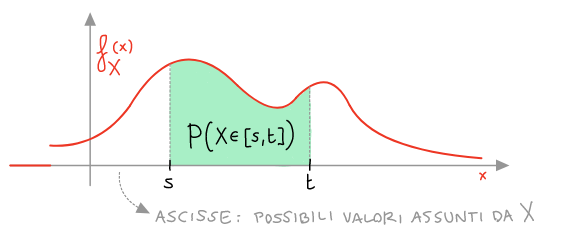
\includegraphics[width=100mm, scale=0.5]{va continue integrale.png}
\end{center}
In altre parole una variabile aleatoria continua può assumere qualunque valore in un
certo intervallo. Esempi di variabile aleatoria continua possono essere il tempo impiegato a
portare a termine un esperimento scientifico o il peso di un individuo.
\\ Ogni v.a. X ha una curva associata. Questa curva, nota come funzione di densità
di probabilità, può essere usata per ottenere le probabilità associate a una v.a.
\\ Visto che \textbf{X assume sempre un valore, otteniamo che l'area totale sottesa dalla curva
deve essere uguale a 1.}
\\ Inoltre visto che l'area sotto il grafico di una funzione di densità di probabilità
tra i punti a e b non varia se gli estremi sono inclusi o esclusi otteniamo che:
\begin{equation*}
    P\{a \leq X \leq b\} = P\{a < X < b \}
\end{equation*}
Questo significa che la probabilità che una variabile aleatoria continua rientri in un
intervallo non cambia se includiamo o no gli estremi.
\\ La curva di densità di probabilità di una v.a. X non scende mai sotto all'asse x ha la
proprietà che l'area delimitata da essa e dall'asse x è sempre uguale a 1.
\\ La curva determina le probabilità di X in questo modo l'area sottesa dalla curva tra i punti a
e b è uguale alla probabilità che X assuma un valore compreso tra a e b.

\subsection*{Analogie tra v.a ass. continua e discreta}
Ci sono analogie formali tra le 2: \begin{itemize}
    \item X ass. continua $P(X \in [s, t]) = \int_{s}^{t} f_x (x) \,dx$ \textbf{Integrale}
    \item X discreta $P(X \in [s, t]) = \sum_{x_i \in [s,t]}p_x (x_i)$ \textbf{Somma}
\end{itemize}
Ma anche importanti differenze!
\\ Se X è assolutamente continua:
\begin{equation*}
    \forall x \in R: P(X=x) = 0
\end{equation*}
\begin{equation*}
    P(X \in [s,t]) = P(X \in (s, t))
\end{equation*}
In particolare: $f_x (x)$ \textbf{NON è} $P(X=x)$, tranne dove $f_x (x) = 0$
\paragraph*{Proprietà} La densità di una v.a. assolutamente continua X è una funzione 
$f_x : R \to R$ (integrabile) tale che: \begin{itemize}
    \item $f_x (x) \geq 0$ $\forall x \in R$
    \item $\int_{-\infty}^{+\infty} f_x (x) \,dx = 1$ Area 
    totale sotto il grafico di $f_x$
\end{itemize}
 \paragraph*{Osservazione} $1 = P(X \in (-\infty, +\infty)) 
 \neq \sum_{x \in (+\infty, -\infty)} P (X = x) = 0$ Dato che $X \in (+\infty, -\infty)$
 è più che numberabile!
 
%Esempio estrazione v.a. uniforme continua
\subsection{Variabile uniforme continua}
Fissiamo un intervallo limitato $[a, b]$ $(-\infty < a < b < -\infty)$.
\\ Una v.a. X si dice uniforme continua in [a, b] e si scrive $X \sim U(a, b)$
se X è ass. cont con densità
\begin{equation*}
    f_x^{x} =
    \begin{cases}
        c \text{ se } x \in [a, b]\\
        0 \text{ se } x \notin [a, b]
    \end{cases} 
\end{equation*}
con $c = \frac{1}{b-a}$
\\ Dato un intervallo $[s, t] \subseteq [a, b]$
\begin{equation*}
    P(X \in [s,t]) = \int_s^t f_x (x) \,dx = 
    \frac{1}{b -a} \int_s^t 1 \,dx = \frac{t-s}{b-a} =
    \frac{\text{Lungh. di } [s,t]}{\text{Lungh. di } [a, b]}
\end{equation*} 
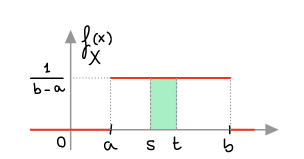
\includegraphics[width=100mm, scale = 0.5]{va unif continua.png}
\paragraph*{Osservazione} Si può mostrare che a partire da una v.a. U(0,1) è possibile
generare una v.a. con distrigià buzione arbitraria!

\paragraph*{Valori assunti da una V.A assolutamente continua}
\begin{equation*}
    X(\Omega) = {x \in R: f_x(x) > 0S}
\end{equation*}

\paragraph{NB} $f_x(x)$ NON è $P(X=x)$, la densitò di una V.A. Continua non è la densità discreta 
e soprattutto NON è la probabilità di assumere il valore x.

\subsection{Valori assunti da una V.A. assolutamente continua}
La densità di una V.A. assolutamente continua X è una funzione $f_x:\mathbb{R} \rightarrow \mathbb{R}$ (integrabile)
tale che:
\begin{equation*}
    f_x(x) \geq 0 \textrm{ } \forall x \in  \mathbb{R}
\end{equation*}
\begin{equation*}
    \int_{-\infty}^{+\infty} f_x(x)  \,dx = 1
\end{equation*}

Le v.a. assolutamente continue sono necessariamente definite su uno spazio campionario
$\Omega$ infinito più che numerabile.

\begin{equation*}
    X(\Omega) = \{ x \in \mathbb{R} : f_x (x) > 0
\end{equation*}

\section{Valore medio e Varianza di V.A. Assolutamente Continue}
Le definizioni di $E[X]$ e $\text{Var}[X]$ per X ass. continua ricalcano quelle date per
v.a. discrete.
\begin{equation*}
    E[X] = \int_{-\infty}^{+\infty} x f_x(x) \,dx 
\end{equation*}
\subsection*{Varianza}
\begin{equation*}
    E[X^2] = \int_{-\infty}^{+\infty} x^2 f_x(x) \,dx
\end{equation*}
Si definisce $SD[X] := \sqrt[]{\text{Var}[X]}$
\paragraph*{Tutte le proprietà valide nelle v.a. discrete continuano a valere}
In particolare:
\begin{equation*}
    E[X+c] = E[X] + c \qquad E[cX] = cE[X] \qquad E[X+Y] = E[X] + E[Y]
\end{equation*}
\begin{equation*}
    \text{Var}[X+c] = \text{Var}[X] \qquad \text{Var}[cX] = c^2 \text{Var}[X]
\end{equation*}
Se X e y \textbf{sono indipendenti}
\section{V.A. Esponenziale}
Misuro il tempo di emissione X di una particella radioattiva da un atomo, con 
"tempo medio di emissione" $\tau$. Sia $\lambda = \frac{1}{\tau}$.
Descriviamo X con una v.a. assolutamente continua:
\begin{equation*}
    f_X(x) =
    \begin{cases}
        \lambda e^{-\lambda x} \quad \text{se} \, x \geq 0 \\
        0 \quad \text{se} \, x < 0 
    \end{cases}
\end{equation*}
Una v.a. X con tale densità è detta Esponenziale di parametro $\lambda \in (0, \infty)$
e si scrive $X \sim \text{Exp}(\lambda)$.
\\ Per ogni intervallo $[s, t] \subseteq [0, \infty]$:
\begin{equation*}
    P(X \in [s, t]) = \int_{s}^{t} f_x(x)\,dx = \int_{s}^{t} \lambda e^{-lambda x}\,dx=
    [- e^{-\lambda x}]_{s}^{t} =
\end{equation*}
\begin{equation*}
    = e^{-\lambda s} - e^{-\lambda t}
\end{equation*}
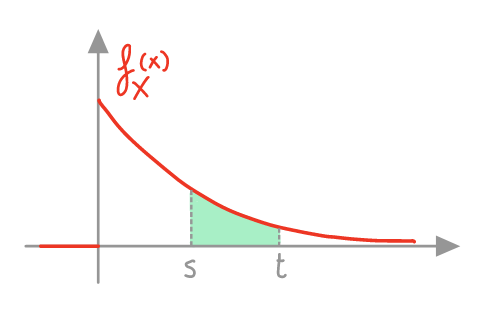
\includegraphics[width=100mm, scale=0.5]{va esponenziale.png}
\section{Funzione di Ripartizione}
Le funzioni di ripartizione ci permettono di capire di che tipo di variabile aleatoria
stiamo parlando.
\begin{equation*}
    F_x (x) = P(X \leq x)
\end{equation*}
A livello probabilistico è la probabilità che X sia minore o uguale a x.
\begin{itemize}
    \item $F_x$ è ben definita per ogni v.a. $X: \Omega \rightarrow \mathbb{R}$, sia che la v.a.
    sia discreta, ass. continua, o nè l'una nè l'altra.
    \item $F_x$ determina la distribuzione della v.a.
    \item $F_x$ è legata alla densità discreta/densità di X
    \begin{equation*}
        F_X(x) = 
        \begin{cases}
        \sum_{x_i \in (- \infty, x]} p_X (x_i) \quad \text{se X è discreta}\\
        \int_{-\infty}^{x} f_x(t)\,dt \quad \text{se X è assolut. continua} 
        \end{cases}
    \end{equation*}
\end{itemize}
La funzione di ripartizione è utile soprattutto per v.a. assolutamente continue, su cui
ci concentreremo nel seguito. Mostriamo comunque un esempio per una v.a. discreta.
\paragraph*{Esempio Bernoulli} Sia $X \sim \text{Be}(p)$ con $p \in (0,1)$.
\begin{equation*}
    X(\Omega) = {0, 1} \qquad p_x{0}=1-p, \qquad p_x(1) = p
\end{equation*}
Allora $F_x(x) = P(X \leq x)$ vale:
\begin{equation*}
    F_X(x) =
    \begin{cases}
        0 \quad \text{se} \quad x < 0 \\
        1-p \quad \text{se} \quad 0 \leq x < 1 \\
        1 \quad se \quad x \leq 1
    \end{cases}
\end{equation*}

\subsection*{Teorema di ripartzione di V.A. Discrete}
\begin{itemize}
    \item X è v.a. discreta $\Leftrightarrow$ $F_x$ è costante a tratti.
    \item Valori assunti{$x_i$} $\Leftrightarrow$ Punti di discontinuità  di $F_x$
    \item Densità discreta $\Leftrightarrow$ Ampiezze dei salti
\end{itemize}
\begin{equation*}
    p_X (x_i) = F_X(x_i) - F_X(X_{\bar{i}})
\end{equation*}
\begin{equation*}
    F_X(x_{\bar{i}}) = \lim_{t \to x_{\bar{i}} F_X(t)}  
\end{equation*}
\subsection*{Funzione di ripartizione di V.A. Assolut. Continue}
X v.a. assolutamente continua $\Leftrightarrow F_X$ è una funzione continua ed
è derivabile a tratti.

\begin{equation}
    \text{Densità} \qquad f_X(x) = (F_X)'(x)
\end{equation}

\section{Variabili aleatorie Normali}
L'ultima classe che vedremo e la più importante, è quella delle variabili aleatorie
normali o Gaussiane.
\\ Una v.a. Z si dice \textbf{Normale Standard} (si scrive $Z \sim N(0,1)$), se è
assolutamente continua con densità:
\begin{equation*}
    f_Z(z)= \frac{1}{\sqrt{2 \pi}} e^{-\frac{z^2}{2}} 
    \quad \forall z \in \mathbb{R}
\end{equation*}
\begin{equation*}
    \rightarrow Z(\Omega) = (-\infty, + \infty)
\end{equation*}
\begin{center}
    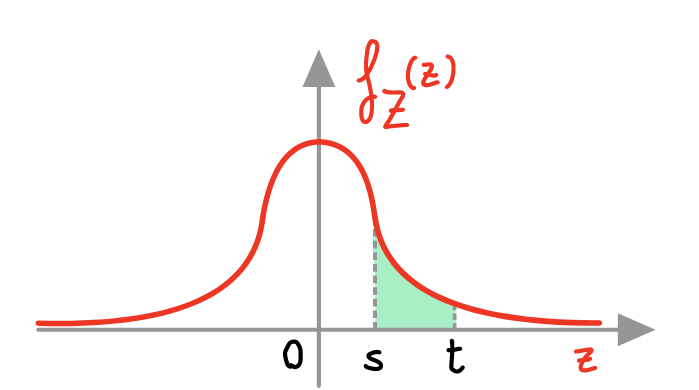
\includegraphics[width=100mm, scale=0.5]{va normale.png}
\end{center}
Come si può notare la forma "a campana" è simmetrica rispetto all'orgine.
\begin{equation}
    \text{"STANDARD"} =
    \begin{cases}
        E[Z] = 0 \\
        \text{Var}[Z] = 1
    \end{cases}
\end{equation}
Dato un intervallo $[s,t] \subseteq \mathbb{R}$
\begin{equation*}
    P(Z\in [s,t]) = \int_{s}^{t} f_z(z)\,dz \qquad 
    \text{(come per ogni v.a. assolutamente continua)}
\end{equation*}
Purtroppo questo integrale non si può calcolare esattamente (la densità $f_Z(z)$
non ammette primitiva esplicita).
\\ Introduciamo la funzione di ripartizione di Z, indicata $\Phi$.
\begin{equation*}
    \Phi(z) = F_Z(z) = P(Z \leq z) = \int_{-\infty}^{z}f_z(t)\,dt
\end{equation*}
Anche questa funzione non di può calcolare esattamente, ma i valori di $\Phi(z)$ per
$z \geq 0$ sono riportati in una tavola.
\\ I valori di $\Phi(z)$ per $z < 0$ si ricavano con la formula
\begin{equation*}
    \Phi(z) = 1 - \Phi(-z)
\end{equation*}
Grazie alla tavola, è come se conoscessimo $\Phi(z) = F_Z(z)$.
Possiamo allora calcolare la probabilità degli intervalli:
\begin{equation*}
    P(Z\in [s,t]) = F_Z(t) - F_Z(s) = \Phi(t) - \Phi(s)
\end{equation*}
Siano ora $\mu \in \mathbb{R}$, $\sigma \in (0, \infty)$.
Una v.a. X si dice \textbf{Normale con media $\mu$ e varianza $\sigma^2$}, si scrive
\textbf{$X \sim N(\mu, \sigma^2)$}, se X è assolutamente continua con
\begin{center}
    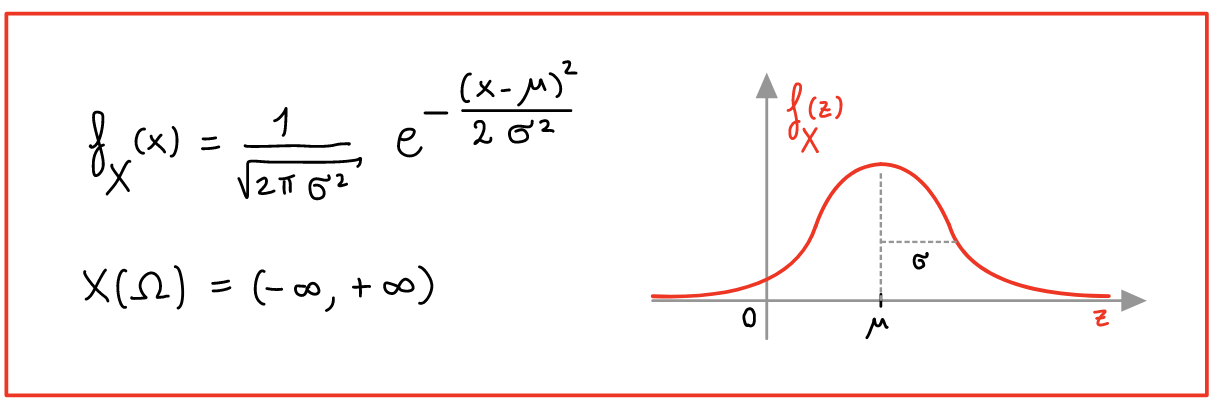
\includegraphics[width=100mm, scale=0.5]{va normale media e var.png}
\end{center}
La densità di $f_X$ di X si ottiene dalla densità di $f_Z$ di $Z \sim N(0,1)$
mediante una traslazione e un riscalamento:
\begin{center}
    $f_X:$ grafico "a campana" centrata in $\mu$, "ampiezza" $\sigma$
\end{center}
Ci si può sempre ricondurre a una v.a. Normale Standard Z:
\begin{equation*}
    X \sim N(\mu, \sigma^2) \rightarrow Z = \frac{X-\mu}{\sigma} \sim N(0,1)
\end{equation*}
\paragraph*{Viceversa}
\begin{equation*}
    Z \sim N(0,1) \rightarrow X = \sigma Z + \mu \sim N(\mu, \sigma^2)
\end{equation*}
Si deduce, in particolare che $\mu$ e $\sigma^2$ sono media e varianza:
\begin{equation*}
    X \sim N(\mu, \sigma^2) \rightarrow E[X] = \mu \quad \text{Var}[X] = \sigma^2
\end{equation*}
Il fatto che ci si può ricondurre a una v.a. normale standard è un caso particolare
della seguente proprietà:
\paragraph*{Teorema} Se X è normale $\rightarrow$ $Y = aX+b$ è normale 
$\forall a \neq 0, b \in \mathbb{R}$
\paragraph*{Teorema} X e Y normali indipendenti $\rightarrow X+Y$ è normale.
\begin{equation*}
    X \sim N(\mu_x, \sigma^{2}_x), \, Y \sim N(\mu_y, \sigma^{2}_y)\, \text{indip.}\,
    \rightarrow X+Y \sim N(\mu_x+\mu_y, \sigma^{2}_x + \sigma^{2}_y)
\end{equation*}
\section*{Vettori Aleatori - Non presenti agli esami}
Completare - vedi commento nel codice
%Dato che non è presente nell'esame sarà compilato alla fine, soprattutto se ci sarà
%il tempo
\section{Legge dei grandi numeri}
Completare - vedi commento nel codice
%Dato che è un tema prettamente teorico verrà scritto alla fine della stesura completa
%degli appunti

% Teoremi di convergenza

\chapter{Teoremi di convergenza}
Siano $X_1, X_2 \dots $ successione di Variabili aleatorie indipendenti identicamente distribuite (V.A I.I.D.).
\\ Discrete $ \rightarrow p_x(x) = p(x) $
\\ Assolutamente continue $ \rightarrow f_{x_i} (x) = f(x) $

Per osservare $X_1, X_2$ devo raccogliere dei dati, il problema è che $p(x), f(x)$ non sono completamente
note. 
\paragraph*{Statistica inferenziale} Dalle osservazioni posso fare delle deduzioni (Inferenze) sulla distribuzione
comune di $X_1, X_2$ ossia su $p(x)$ e $f(x)$.
\\ Non posso osservare tutte le V.A per questo ne scelgo casualmente n. 
\\ $X_1, \dots ,X_n$ Campione aleatorio di ampiezza n. Lavoreremo con variabili aleatorie che siano funzioni del 
campione aleatorio, cioè del tipo $g(x_1, \dots ,x:n)$
\paragraph*{Statistica campionaria} Dato un campione aleatorio $X_1, \dots, X_n$ una statistica campionaria
è una qualunque funzione del campione:
\begin{equation*}
    g(X_1, \dots, X_n) \text{   } (g:\mathbb{R}^n\rightarrow\mathbb{R})
\end{equation*}

\paragraph*{Esempio di statistica campionaria} Media campionaria
\begin{equation*}
    \bar{X_n}:\frac{1}{n}\sum_{n=1}^n X_i
\end{equation*}
\section{Distribuzione di X}
\begin{equation*}
    \mathbb{P} (a  < \bar{X_nx} \leq b) = \mathbb{P} (\frac{a - \mu}{\frac{\sigma}{\sqrt{n}}} 
    < \frac{X_n - \mu}{\frac{\sigma}{\sqrt{n}}} \leq \frac{b - \mu}{\frac{\sigma}{\sqrt{n}}})   
\end{equation*}
\begin{equation*}
    \text{Var}(\bar{X_n}) = \frac{\sigma ^ 2}{n} 
\end{equation*}
\begin{equation*}
    \frac{\sigma}{\sqrt{n}} = \sqrt{\text{Var}}
\end{equation*}

\section{Teorema del limite centrale}
Siano $X_1, ..., X_n$ v.a i.i.d. (Variabili aleatorie indipendenti identicamente distribuite)
$E(i) = \mu$ e $\text{Var}X_i = \sigma^2$ (con media e varianza finite).
\begin{equation*}
    \mathbb{P} (\frac{X_n-\mu}{\frac{\sigma}{\sqrt{n}}} \leq t) \rightarrow \Phi (t) \quad n \rightarrow + \infty   
\end{equation*}
Dove $\Phi$ è la funzione di ripartizione di una V.A $Z\sim N(0,1)$
\begin{equation*}
    \Phi(t) = \mathbb{P}(Z \leq t)
\end{equation*}
\paragraph*{Condizione per usare l'approssimazione normale} Abbiamo definito 
che solo con $n \geq 30$ si può usare l'approx per semplicità, in realtà non è semplice
dare un criterio univoco dato che dipende dall'asimmetria del campione di partenza.
\paragraph*{Nota per i campioni discreti} Quando ho un campione discreto è sempre necessario
applicare la correzione di continuità 
%https://it.wikipedia.org/wiki/Standardizzazione_(statistica)

\section*{Note per esercizi}
\begin{itemize}
    \item Riconosci la distribuzione notevole
    \item Ricava media e Var
    \item Scrivi la formula che ti serve (es P che una va sia $\leq$ di n)
    \item Effettua la correzione di continuità se si tratta di una VA discreta
    \item Verifica se $n\geq 30$, questo per verificare se si può applicare il TLC (teorema del limite centrale)
    \item Sottrai media e dividi per $\sqrt{\text{Var}}$
    \item Se hai > come segno, anzichè $\mathbb{P}$ dovrai trovare $1-\mathbb{P}$ e invertire il segno in <
    \item Se trovi un valore $z$ negativo all'interno di $\Phi(z)$ dovrai calcolare $1 - \Phi(-z)$, quindi rendere positivo
    z, calcolare il suo $\Phi$ e sottrarlo a 1
\end{itemize}

\chapter{Stima di parametri}
In questo capitolo vedremo come usare i dati campionari per stimare una media,
una varianza o una proporzione della popolazione. Verranno discusse le stime puntuali
che sono stime a valore singolo del parametro. Verrà considerato poi l'errore standard di
queste stime. Inoltre considereremo gli intervallo di confidenza, che contengono il parametro
con un certo livello di confidenza.
\section{Statistica inferenziale}
La \textbf{statistica inferenziale} ha lo scopo di definire in modo non ambiguo e
quantitativo la plausibilità di un'inferenza.
\\ La plausibilità di un'inferenza dipende dal modo con cui è stato selezionato
il campione di n individui della popolazione.
La corretta metodologia di campionamento è la \textbf{scelta casuale}.
\\ Per la casualità dle campionamento utilizzo il calcolo delle probabilità.
\\ Quando parleremo di popolazione tratteremo sempre N molto grandi rispetto alla numerosità
del campione. 
\paragraph*{Popolazione} V.A. i.i.d. con la stessa distribuzione $\leftrightarrow$
legge F.
\\ Consideriamo il caso in cui F è nota a meno di qualche parametro incongito.
\paragraph*{Modello statistico parametrico} Famiglia di leggi note a meno di uno o
più parametri.
\begin{itemize}
    \item Caso discreto: $p(x; \Theta) \quad$ 
    Densità discreta $p(x;\Theta):\mathbb{P}_\Theta (X=x)$
    \item Caso continuo: densità $f(x; \Theta)$
\end{itemize}
\paragraph*{Attenzione} Non confondere le V.A. con le osservazioni
\begin{itemize}
    \item $X_1, ..., X_n \quad$ sono le v.a.
    \item $x_1, ..., X_n \quad$ sono le osservazioni
\end{itemize}
\paragraph*{Esempi di modelli statistici}
Esempi di modelli statistici sono:
\begin{itemize}
    \item Modello di Bernoulli
    \item Modello esponenziale
    \item Modello normale
\end{itemize}
Dato $(X_1, ..., X_n)$ campione casuale, si definisce \textbf{Statistica} una
funzione del campione, ossia una v.a. T della forma
\begin{equation*}
    T=f(X_1, ..., X_n)
\end{equation*}
\paragraph*{Esempi di statistiche}
\begin{itemize}
    \item $\bar{X}_n = \frac{X_1+...+X_n}{n} \quad$ Media campionaria (v.a.)
    \item $S^{2}_n = \frac{1}{n-1} \sum_{i=1}^n(X_i - \bar{X}_n)^2 \quad$ Varianza campionaria (v.a.)
\end{itemize}
\section{Statistica parametrica e Stimatori} 
Il primo obiettivo della statistica inferenziale è fornire una stima dei
parametri incogniti.   
\paragraph*{Stimatori} Uno \textbf{Stimatore} è una statistica il cui valore
dipende dal particolare campione che è stato estratto. Il valore dello stimatore,
\textbf{la Stima}, viene usato per predire il valore di un parametro della popolazione.
particolari statistiche che servono a stimare i parametri incogniti.
\paragraph*{Stimatori Puntuali} Sono valori singoli che speriamo siano prossimi
ai parametri stimati.
\paragraph*{Stimatori intervallari} Meglio noti come \textbf{Intervalli di confidenza},
in questo caso non rappresentano un singolo valore, ma un intervallo in cui ci
aspettiamo che il parametro rientri. Ci occupiamo anche di determinare quanta
confidenza associare a un dato intervallo, cioè quanto possiamo essere sicuro che il parametro
si trovi in questo intervallo.
\paragraph*{Definizione Stimatore Corretto} Uno \textbf{Stimatore} T si dice \textbf{Non Distorto o Corretto}
se:
\begin{equation*}
    \mathbb{E}_\Theta{T}: \mathbb{E}_\Theta(g(X_1, ..., X_n)) = \Theta
\end{equation*}
Dove $E_\Theta$ è il valore medio rispetto alla probabilità di $P_\Theta$.
\paragraph*{In parole povere} Uno stimatore il cui valore atteso è uguale al parametro
che si vuole stimare si dice \textbf{corretto} per quel parametro.
\paragraph*{$\bar{X}_n$ è lo stimatore non distorto di}
\begin{itemize}
    \item p in un modello di Bernoulli
    \item $\lambda$ in un modello di Poisson
    \item $\frac{1}{\lambda}$ in un modello esponenziale
    \item $\mu$ in un modello normale
\end{itemize}
\paragraph*{Osservazione} La proprietà di essere non distorto NON è stabile per
trasformazioni, ad esempio nel modlelo esponenziale $X_n$ è stimatore non distorto
di $\frac{1}{\lambda}$, ma si ha che $\frac{1}{\bar(X)_n}$ NON è uno stimatore non
distorto di $\lambda$.
\paragraph*{Stimatore consistente} Uno stimatore non distorto di $\Theta$ si dice
\textbf{Consistente} se, quando $n \rightarrow + \infty$
\begin{equation*}
    \text{Var}_\Theta (T) \rightarrow 0
\end{equation*}
Quando abbiamo un campione casuale estratto da una popolazione con media $\mu$
e varianza $\sigma^2$ finite si ha sempre che $\bar{X}_n$ \textbf{è uno stimatore consistente
di $\mu$}:
\begin{equation*}
    \text{Var}_\sigma(\bar{X}_n) = \frac{\sigma^2}{n} \rightarrow 0 \quad n \rightarrow + \infty
\end{equation*}
\\ Stimatore di $\Theta = g(X_1, ..., X_n) \rightarrow$ V.A.
\\ Stima di $\Theta: f(x_1, ..., X_n) \rightarrow$ Numero.
\\ Stima di $\mu$ per un campione casuale $X_1, ..., X_n$ di cui osserviamo
$x_1, ..., x_n$.
\begin{equation*}
    \hat{\mu} = \bar{x}_n = \frac{x_1+...+x_n}{n}
\end{equation*}
\section{Errore standard}
Supponiamo di considerare un campione casuale con media $\mu$ incognita
e varianza $\sigma$ nota:
\begin{equation*}
    \text{Var}\bar{X}_n= \frac{\sigma^2}{n}
\end{equation*}
\begin{equation*}
    \text{SD}(\bar{X}_n) = \frac{\sigma}{\sqrt{n}} \quad \text{deviazione standard SD}
\end{equation*}
Se si pensa $\bar{X}_n$ come stimatore di $\mu$, SD$(\bar{X}_n)$ prende il nome Di
\textbf{errore standard}, esso rappresenta l'errore commesso stimando $\mu$ con $\bar{X}_n$.
\\ Ora consideriamo un modello statistico con \textbf{varianza incognita}.
\\ In statistica descrittiva: siano n osservazioni $(x_1, ..., x_n)$;
\begin{equation*}
    s^{2}_n=\frac{1}{n-1}\sum_{k=1}^n(x_k-\bar{x}_n)^2
\end{equation*}
\'E sensato introdurre in un modello statistico con varianza $\sigma^2$ incognita lo
stimatore
\begin{equation*}
    S^{2}_n=\frac{1}{n-1}\sum_{k=1}^n(X_k-\bar{X}_n)^2
\end{equation*}
Se nel modello statistico con varianza $\sigma^2$ incognita \textbf{la media è nota}, si ha che
lo stimatore:
\begin{equation*}
    \bar{S}^{2}_n = \frac{1}{n}\sum_{i=1}^n(X_u - \mu)^2
\end{equation*}
è uno stimatore corretto di $\sigma^2$.
\section{Chi quadrato}
\subsection*{Distribuzione delle statistiche campionarie}
\paragraph*{Campione normale}
$X_1, ..., X_n$ campione casuale $\mathcal{N}(\mu, \sigma^2)$
\begin{equation*}
    \bar{X}_n \sim \mathcal{N}(\mu, \frac{\sigma^2}{n})
\end{equation*}
Standardizzando otteniamo
\begin{equation*}
    \frac{\bar{X}_n-\mu}{\frac{\sigma}{\sqrt{n}}} \sim \mathcal{N}(0,1)
\end{equation*}
Per caratterizzare la legge di $S_{n}^2$ e di $\bar{S}_{n}^2$ dobbiamo
introdurre una nuova distribuzione continua
\begin{equation*}
    \chi^2(n)
\end{equation*}
Si dice legge \textbf{chi quadrato con n gradi di libertà} la legge di una v.a.
\begin{equation*}
    Y = \sum_{i=1}^n Z_{i}^2 \,, \quad z_1, ..., z_n \quad \text{i.i.d.}\quad \mathcal{N}(0,1)
\end{equation*}
%Video Lezione 10 T1 minuto 32:29 - https://elearning.unimib.it/mod/kalvidres/view.php?id=926811
Dove Y è una v.a. $\geq 0$ con densità $f_r(t) = c_n t^{\frac{n}{2}-1} e^{-\frac{t}{2}} 
\qquad \text{per} \quad t>0$
\\ Si ha $\mathbb{E}(Y) = n$ e $\text{Var}(Y)=2n$
\\ Per $n = 2$ è la legge $\text{exp}(\frac{1}{2})$
\\ Per n grande vale l'approssimazione della legge $\chi^2(n)$ con una
$\mathcal{N}(n,2n)$
\paragraph*{Proposizione} Sia $(X_1, ..., X_n)$ campione casuale estratto
da una popolazione $\mathcal{N}(\mu, \sigma^2)$.
\begin{enumerate}
    \item $\sum_{i=1}^n(\frac{X_i-\mu}{\sigma})^2 \sim \chi^2(n)$
    \item $\sum_{i=1}^n(\frac{X_i-\bar{X}_n}{\sigma}) \sim \chi^2(n-1)$
    \item se $S_{n}^2 = \frac{1}{n-1}\sum_{i=1}^n(X_i - \bar{X}_n)^2$
    \\ $(n-1)\frac{S_{n}^2}{\sigma^2} \sim \chi^2(n-1)$
    \item $S_{n}^2$ e $\bar{X}_n$ sono indipendenti
\end{enumerate}
Riassumendo $\chi^2$ ci serve per la distribuzione della legge delle varianze campionarie
\section{Distribuzione t di student}
\paragraph*{Definizione Wikipedia} 
Nella teoria delle probabilità la distribuzione di Student, o t di Student, 
è una distribuzione di probabilità continua che governa il rapporto tra due variabili aleatorie, 
la prima con distribuzione normale e la seconda, al quadrato, segue una distribuzione chi quadrato.
\\ Questa distribuzione interviene nella stima della media di una popolazione che segue la distribuzione normale, 
e viene utilizzata negli omonimi test t di Student per la significatività e per ogni intervallo 
di confidenza della differenza tra due medie. 
\paragraph*{Definizione matematica}Si dice legge di \textbf{t di student con n gradi di libertà} la legge di una v.a.
\begin{equation*}
    T = \frac{z}{\sqrt{\frac{Y}{n}}}
\end{equation*}
\begin{equation*}
    z \sim \mathcal{N}(0,1)
\end{equation*}
\begin{equation*}
    Y \sim \chi^2(n)
\end{equation*}
Z e Y sono indipendenti.
\begin{equation*}
    \mathbb{E}(T)=0 \quad \text{Var}[T] = 1
\end{equation*}
T è una v.a. continua con densità
\begin{equation*}
    f_T(t) = c_n(1+\frac{t^2}{n})^{\frac{-(n+1)}{2}}
\end{equation*}
$c_n$ è una costante che fa risultare l'integrale della $f = 1$.
\paragraph*{Proposizione} Sia $X_1, ..., X_n$ un campione casuale estratto da
una popolazione $\mathcal{N}(\mu, \sigma^2)$. Allora
\begin{equation*}
    \frac{\bar{X}_n-\mu}{\sqrt{\frac{s^2_{n}}{n}}} \sim t(n-1)
\end{equation*}
\section{Parte pratica}
Cosa dovremo saper calcolare di queste variabili aleatorie? I loro percentili.
\\ X v.a.
\\ $P(X\leq q_\alpha) = \alpha$ Fissato $\alpha$, trovare $q_\alpha$.
\\ $q_\alpha$ = $\alpha$ - esimo quantile o $100\alpha$ - percentile di X.
\begin{itemize}
    \item $Z \sim \mathcal{N}(0,1) \qquad z_\alpha$ t.c. $\mathbb{P}(Z>z_\alpha) = \alpha$
    \item $T \sim t(n) \qquad t_{\alpha, n}$ t.c. $\mathbb{P}(T>t_{\alpha, n}) = \alpha$
    \item $Y \sim \chi^2{n} \qquad \chi^2_{\alpha, n}$ t.c. $\mathbb{P}(Y>\chi^2_{\alpha,n}) = \alpha$
    \item $z_\alpha$, $t_{n, \alpha}$, $\chi^2_{m, \alpha} 
    \qquad 100(1-\alpha) \text{percentili} \quad (\text{di}\quad Z, T, Y)$
\end{itemize}
\begin{equation*}
    Z \sim \mathcal{N}(0,1) \qquad \alpha \quad \text{definito da}
\end{equation*}
\begin{gather*}
    P(Z>z_\alpha) = \alpha \\
    P(Z\leq Z_\alpha) = 1-\alpha \\
    z_\alpha = 100(1-\alpha) \qquad \text{percentili di Z}\\
    z_\alpha = \Phi^{-1}{1-\alpha} \\
    P(Y > X^2_{\alpha, n}) = \alpha
\end{gather*}
La simmetria di T student è la stessa della normale.
\\ Mentre per la $\chi^2$ non ci sono simmetrie.
\begin{center}
    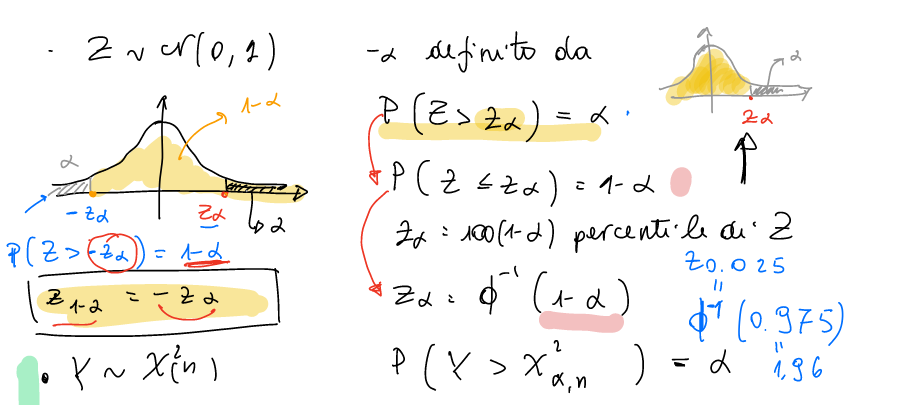
\includegraphics[width=120mm,scale=0.5]{Simmetria t di student.png}
\end{center}






\end{document}